\chapter{Applicazioni lineari}
\section{Definizione}
\begin{definizione} \label{d:applicazione-lineare}
	Siano $V$ e $Z$ due spazi vettoriali su un campo $K$.
	Si definisce \emph{applicazione lineare} una funzione $T\colon V\to Z$ omogenea e additiva, ossia per la quale $\forall  x,  y\in V$ e $\lambda\in K$, si ha
	\begin{equation*}
		T(x+y)=T(x)+T(y)\qeq T(\lambda x)=\lambda T(x),
	\end{equation*}
	dove i primi membri delle uguaglianze sono operazioni in $V$, e i secondi sono operazioni in $Z$ (indicando con $+$ e $\cdot$ le due operazioni interne per entrambi gli spazi).
\end{definizione}
Le applicazioni lineari sono dunque degli omomorfismi tra spazi vettoriali, in quanto ne preservano la struttura data dalle operazioni interne.
Per linearità, vale sempre la relazione $T(0_V)=0_Z$, poiché $T(0_V)=T(0_V+0_V)=T(0_V)+T(0_V)$, da cui $T(0_V)=0_Z$ sottraendo $T(0_V)$ a entrambi i membri: quest aè una condizione facile da usare per verificare la linearità di una data funzione.
L'insieme delle applicazioni lineari da $V$ a $Z$ è indicato con $\lin(V,Z)$.
Un'applicazione lineare da uno spazio in s\'e stesso è detta \emph{endomorfismo} (lineare), e indichiamo l'insieme degli endomorfismi di uno spazio $V$ con $\End(V)$.

\paragraph{Esempi}
\begin{itemize}
	\item L'applicazione identità di $V$, indicata con $\id_V$, per la quale $\id_V(v)=v$ per ogni $v\in V$, è ovviamente lineare.
	\item L'applicazione nulla, che associa ad ogni elemento lo zero dello spazio di arrivo: $0(v)=0_Z$ per ogni $v\in V$, anch'essa lineare in modo ovvio.
	\item Sia $W$ un sottospazio di $V$: chiamiamo \emph{proiezione canonica} in $W$ la funzione $\pi\colon V\to V\quot W$ che ad ogni $v\in V$ associa la classe di equivalenza $[v]_W=W+v$.
		Tale funzione è additiva in quanto per $a,b\in V$, $\pi(a+b)=W+(a+b)=(W+a)+(W+b)=\pi(a)+\pi(b)$.
		È anche omogenea perch\'e $\pi(\lambda a)=W+\lambda a=\lambda(W+a)=\lambda\pi(a)$.
		La funzione $\pi$ è quindi un'applicazione lineare.
	\item La funzione $f\colon\R^2\to\R^2$ data da $f([x,y]^T)=[x+y,y+1]^T$ non è un'applicazione lineare, poich\'e $f([0,0]^T)=[0,1]^T\ne[0,0]^T$.
\end{itemize}

L'iniettività e la suriettività delle applicazioni lineari sono definite allo stesso modo di una qualsiasi funzione.
In particolare, un'applicazione lineare che è sia iniettiva che suriettiva è detta \emph{isomorfismo lineare} (o solo isomorfismo).
Due spazi vettoriali $V$ e $Z$ legati da un isomorfismo $T\colon V\to Z$ sono detti \emph{isomorfi}, e si indica ciò con la scrittura $V\cong Z$.

Come ogni omomorfismo, definiamo un nucleo anche per le applicazioni lineari.
\begin{definizione} \label{d:nucleo-applicazione-lineare}
	Si definisce \emph{nucleo} dell'omomorfismo $T$ l'insieme degli elementi $x\in V$ tali per cui $T(x)=0_Z$:
	\begin{equation*}
		\Ker T=\{x\in V\colon T(x)=0_Z\}.
	\end{equation*}
\end{definizione}
La linearità permette una facile verifica dell'iniettività di un'applicazione lineare.
\begin{teorema} \label{t:iniettivita-nucleo}
	Un'applicazione lineare $T\in\lin(V,Z)$ è iniettiva se e solo se $\Ker T=\{0_V\}$.
\end{teorema}
\begin{proof}
	Per ogni applicazione lineare vale $T(0_V)=0_Z$, come già visto.
	Per l'iniettività, ogni $z\in Z$ ha un'unica controimmagine, quindi l'unico $v\in V$ per cui $T(v)=0_Z$ è proprio $0_V$, di conseguenza $\Ker T=\{0_V\}$.

	Viceversa, ipotizziamo $\Ker T=\{0_V\}$.
	Se $T(v)=T(w)$ allora $T(v)-T(w)=0_Z$, e per linearità si ha $T(v-w)=0_Z$, cioè $v-w\in\Ker T$.
	Ma $\Ker T=\{0_V\}$ implica $v-w=0_V$, dunque $v=w$ e $T$ è iniettiva.
\end{proof}
Le applicazioni lineari conservano anche i rapporti tra sottospazi: dati $W,U$ sottospazi se $W\leq V$, e $T\colon V\to Z$, allora $T(W)\leq Z$; analogamente le controimmagini di $U\leq Z$ sono $T^{-1}(U)\leq V$.
Ad esempio, siano $  y_1,  y_2\in T(W)$.
Essi certamente hanno le loro controimmagini in $W$: siano esse $  w_1,  w_2\in W\colon T(  w_1)=  y_1$ e $T(  w_2)=  y_2$.
Allora $T(  w_1+  w_2)=T(  w_1)+T(  w_2)=  y_1+  y_2\in T(W)$, poiché $  w_1+  w_2\in W$ dato che è uno spazio vettoriale.
Analogamente, dati $  y\in T(W)$ e $  w\in W$ per i quali $T(  w)=  y$, si ha $T(\lambda  w)=\lambda T(  w)=\lambda  y\in T(W)$.
Inoltre poiché $\{0_Z\}\leq Z$, si ha che $\Ker T\leq V$.

\begin{definizione} \label{d:immagine-applicazione-lineare}
	Sia $T\in\lin(V,Z)$.
	Si definisce \emph{immagine} di $T$ l'insieme degli elementi $  z\in Z$ per i quali esiste una controimmagine $  v\in V$:
	\begin{equation*}
		\Imm T=\{  z\in Z\colon\exists   v\in V\colon T(  v)=  z\}.
	\end{equation*}
\end{definizione}
Sia il nucleo che l'immagine di un omomorfismo $T\in\lin(V,Z)$ sono sottospazi vettoriali, rispettivamente di $V$ e di $Z$.
Infatti:
\begin{itemize}
	\item Siano $  v,  w\in\Ker T$ e $k\in K$.
		Allora $T(  v+  w)=T(  v)+T(  w)=0_V+0_V=0_V$, e $T(k  v)=kT(  v)=k0_V=0_V$, quindi $  v+  w$ e $k  v$ appartengono a $\Ker T$.
	\item Siano $  y,  z\in\Imm T$ e $k\in K$.
		Esistono due vettori $  a,  b\in V$ per i quali $T(  a)=  y$ e $T(  b)=  z$.
		Allora $  z+  y=T(  a)+T(  b)=T(  a+  b)$, cioè $  z+  y$ è l'immagine di un elemento $  a+  b$, che appartiene $V$ che è uno spazio vettoriale; analogamente $T(k  a)=kT(  a)=k  y$, quindi $k  y$ è a sua volta l'immagine di un elemento $k  a\in V$.
		Di conseguenza $  z+  y$ e $k  y$ appartengono ancora a $\Imm T$.
\end{itemize}

\section{Teoremi degli isomorfismi}
Il seguente teorema è importante perché consente di esprimere l'immagine di un omomorfismo come somma di un elemento del suo nucleo e di una sua immagine.
\begin{teorema}
	Siano $T\in\lin(V,Z)$ e $  z$ un elemento di $Z$ per cui $T(x)=z$, con $  x\in V$.
	La classe di equivalenza $\Ker T+  x$ è l'insieme degli elementi $  y$ di $V$ che sono controimmagini di $  z$:
	\begin{equation*}
		V/ \Ker T = \Ker T+  x=\{  y\in V\colon T(  y)=  z\}.
	\end{equation*}
\end{teorema}
\begin{proof}
	Un elemento della classe $\Ker T+  x$ è del tipo $\alpha+  x$, con $\alpha\in\Ker T$.
	La sua immagine è $T(\alpha+  x)=T(\alpha)+T(  x)=0_Z+T(  x)\in Z$, quindi $\Ker T+  x\subseteq\{  y\in V\colon T(  y)=  z\}$.

	Sia invece $  y\in V$, tale che $T(  y)=  z$: questo elemento appartiene a $\Ker T+  x$, e si può sempre esprimere come $y=\beta+  x$ con $\beta\in\Ker T$.
	Allora $T(  y)=T(\beta)+T(  x)=0_Z+T(  x)$; posti $T(  x)=T(  y)=  z$, si ha $T(  x)-T(  y)=0_Z$, ossia $  x-  y\in\Ker T$: allora $\exists\beta\in\Ker T$ per cui $  x-  y=\beta$, oppure $  y=  x+\beta$, cioè ogni $  y$ avente un'immagine in $Z$ tramite $T$ appartiene al laterale $\Ker T+  x$.
	Quindi, poiché i due insiemi si includono a vicenda, devono coincidere.
\end{proof}
\begin{teorema} \label{t:dimensione-quoziente}
	Sia $W\leq V$ con $V$ di dimensione finita.
	La dimensione di $V/W$ è finita e vale $\dim V-\dim W$.
\end{teorema}
\begin{proof}
	Il sottospazio $W$ ha certamente dimensione finita: sia $\{  e_i\}_{i=1}^n$ una base di $W$.
	Essa si può estendere ad una base di V, per il teorema \ref{estensione-base}.
	Allora $E=\{  e_1,  e_2,\dots,  e_n,  f_{n+1},\dots,  f_{n+m}\}$ è una base di $V$.
	Ora, prendiamo $W+  a$, e $  a\in V$ si può scrivere come combinazione lineare degli elementi di $E$: $  a=\lambda_1  e_1+\lambda_2  e_2+\dots+\lambda_n  e_n+\lambda_{n+1}  f_{n+1}+\dots+\lambda_{n+m}  f_{n+m}$.
	Poiché i termini fino a $\lambda_n  e_n$ individuano un elemento di $W$, si ha che $a=W+\mu_1  f_{n+1}+\dots+\mu_m  f_{n+m}$.
	Per la definizione della somma $\oplus$, questo è equivalente ad $a=\mu_1(W+  f_{n+1})\oplus\dots\oplus\mu_m(W+  f_{n+m})$, ma allora la famiglia $\{W+  f_{n+i}\}_{i=1}^m$ è un sistema di generatori di $W$, avente ovviamente $m$ elementi.
	Una combinazione lineare di questa base può essere allora nulla se e solo se tutti i coefficienti sono nulli: sia quindi
	\begin{equation*}
		\lambda_1(W+  f_{n+1})\oplus\lambda_2(W+  f_{n+2})\oplus\dots\oplus\lambda_m(W+  f_{n+m})=0_{V/W}=W+0_V.
	\end{equation*}
	Essa è per definizione equivalente a $W+(\lambda_1  f_{n+1}+\dots+\lambda_m  f_{n+m})$.
	Per l'uguaglianza precedente, quindi, deve essere $\lambda_1  f_{n+1}+\dots+\lambda_m  f_{n+m}=0_V$, ma dato che l'insieme $\{  f_{n+i}\}_{i=1}^m$ è linearmente indipendente, questo può accadere se e solo se tutti i $\lambda_i$ sono nulli.
	Quindi anche l'insieme $\{W+  f_{n+i}\}_{i=1}^m$ è linearmente indipendente, e poiché genera $V/W$ è una base di $V/W$, che quindi ha dimensione $m$.
\end{proof}
\begin{teorema}
	Sia $T\in\lin(V,Z)$ e $\{  e_i\}_{i\in I}\subset V$.
	Allora:
	\begin{enumerate}
		\item Se $\{  e_i\}_{i\in I}$ è un sistema di generatori per $V$ e $T$ è suriettivo, allora $\{T(  e_i)\}_{i\in I}$ è un sistema di generatori per $Z$;
		\item Se $\{  e_i\}_{i\in I}$ è un sistema linearmente indipendente e $T$ è iniettivo, allora $\{T(  e_i)\}_{i\in I}$ è linearmente indipendente in $Z$.
	\end{enumerate}
\end{teorema}
\begin{proof}
	Sia $  z\in Z$: poiché $T$ è suriettivo, esiste $  v\in V$ per cui $T(  v)=  z$.
	Allora dato che $  v$ è dato da una combinazione lineare di elementi del sistema di generatori, cioè $  v=\lambda_1  e_1+\lambda_2  e_2+\dots+\lambda_r  e_r$, con $\lambda_i\in K$ e $\{  e_1,  e_2,\dots,  e_r\}\subset\{  e_i\}_{i\in I}$, si ha che $  z=T(  v)=\lambda_1T(  e_i)+\dots+\lambda_rT(  e_r)$, quindi $\{T(  e_1),\dots,T(  e_r)\}$ è un sistema di generatori per $Z$.

	Sia ora $I_0$ un sottoinsieme di cardinalità finita di $I$.
	Presa una combinazione lineare che dia $0_Z$, per la linearità dell'operazione $T$ si ha
	\begin{equation*}
		\sum_{j\in I_0}\lambda_jT(  e_j)=T\big(\sum_{j\in I_0}\lambda_j  e_j\big)=0_Z.
	\end{equation*}
	Questo significa che $\sum_{j\in I_0}\lambda_j  e_j\in\Ker T$, ma poiché $T$ è iniettivo il suo nucleo è composto dal solo $0_V$.
	Allora $\sum_{j\in I_0}\lambda_j  e_j=0_V$, e dato che $\{  e_i\}_{i\in I_0}$ è un sistema linearmente indipendente ciò può accadere se e solo se $\forall j\in I_0$ $\lambda_j=0_K$. Quindi $\{T(  e_j)\}_{j\in I_0}$ è un sistema linearmente indipendente.
\end{proof}
Dunque combinando le due affermazioni risulta che l'immagine di una base tramite un isomorfismo è una base per lo spazio di arrivo.

\begin{teorema}[Primo teorema dell'isomorfismo] \label{t:primo-isomorfismo}
	Sia $T\in\lin(V,Z)$.
	Esiste ed è unico un omomorfismo iniettivo $\tilde{T}\in\lin(V\quot\Ker T,Z)$ tale che $\tilde{T}\circ\pi=T$, dove $\pi$ è la proiezione canonica da $V$ in $V\quot\Ker T$.
	Allora $V\quot\Ker T\cong\Imm T$.
	\begin{figure}[h!]
		\centering
		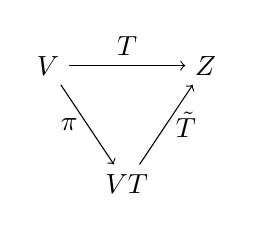
\begin{tikzpicture}
			\node (V) at (-1,1.5) {$V$};
			\node (Z) at (1,1.5) {$Z$};
			\node (K) at (0,0) {$V\quot\Ker T$};
			\draw [->] (V) to node[above]{$T$} (Z);
			\draw [->] (V) to node[left]{$\pi$} (K);
			\draw [->] (K) to node[right]{$\tilde{T}$} (Z);
		\end{tikzpicture}
	\end{figure}
\end{teorema}
\begin{proof}
	Verifichiamo che l'applicazione è ben definita, ossia che non dipenda dal rappresentante scelto per le classi in $V\quot\Ker T$, dimostriamo poi la linearità e infine l'iniettività.

	Gli elementi di $V\quot\Ker T$ sono del tipo $\Ker T+  a$, e la proiezione canonica $\pi$ manda $  a$ in $\Ker T+  a$.
	Deve quindi risultare $\tilde{T}\big(\pi(  a)\big)=\tilde{T}(\Ker T+  a)=T(  a)$.
	Affinché $\tilde{T}$ sia ben definito, se $\Ker T+  a=\Ker T+  b$ deve essere $T(  a)=T(  b)$.
	Questo è mostrato applicando $T$ all'uguaglianza, e la seconda segue automaticamente per la linearità di $T$, oppure notando che $  a\sim  b$ quando $  a-  b\in\Ker T$, e in tal caso $0_Z=T(  a-  b)=T(  a)-T(  b)$ cioè $T(  a)=T(  b)$.
	Se poi $\Ker T+  a$ e $\Ker T+  b$ sono distinte, si ha $  a+  b\notin\Ker T$: sia quindi per assurdo che $\tilde{T}(\Ker T+  a)=\tilde{T}(\Ker T+  b)$, cioè per definizione dell'applicazione lineare $\tilde{T}$ che $T(  a)=T(  b)$, che è in contraddizione con quanto ipotizzato in precedenza.
	Quindi l'applicazione esiste unica.

	Si considerino le due classi di $V\quot\Ker T$ con rappresentante $  a$ e $  b$: applicando $\tilde{T}$ alla loro somma (come definita nel capitolo \ref{sec:spazi_quoziente}) si ottiene
	\begin{equation}
		\tilde{T}[(\Ker T+  a)\oplus(\Ker T+  b)]=\tilde{T}(\Ker T+  a)+\tilde{T}(\Ker T+  b)=T(  a)+T(  b),
	\end{equation}
	e allo stesso tempo
	\begin{equation}
		\tilde{T}[(\Ker T+  a)\oplus(\Ker T+  b)]=\tilde{T}[\Ker T+(  a+  b)]=T(  a+  b)=T(  a)+T(  b).
	\end{equation}
	perciò $\tilde T$ è lineare.

	Consideriamo il $\Ker \tilde{T}$: esso è definito da
	\begin{equation*}
		\Ker \tilde{T} = \{\Ker T +  v\in V/\Ker T\colon T(  v) = 0 \}.
	\end{equation*}
	Si ha quindi che $\Ker \tilde{T}$ si riduce al solo $\Ker T$ e per come $\tilde{T}$ è definita questo si riduce al solo zero.
	Ciò prova che $\tilde{T}$ è iniettiva.
	Inoltre, $T(V)$ è anche automaticamente suriettiva poichè tutti gli elementi su cui agisce $T$ sono queli su cui agisce anche $\tilde{T}$), dunque $\tilde{T}$ è un isomorfismo: allora $V\quot\Ker T\cong\Imm T$.
\end{proof}
\begin{corollario}
	Se $V$ ha dimensione finita e $T\in\lin(V,Z)$, allora $\dim V=\dim\Ker T+\dim\Imm T$.
\end{corollario}
\begin{proof}
	Segue facilmente dal teorema precedente e dal \ref{t:dimensione-quoziente}.
\end{proof}

\begin{teorema}[Secondo teorema dell'isomorfismo]
	Siano $W,Z$ sottospazi vettoriali di $V$.
	Allora $(W+Z)\quot Z$ e $W\quot(W\cap Z)$ sono isomorfi per mezzo dell'applicazione lineare $T$ definita come $T\colon Z+(  w +   z)\mapsto Z\cap W+  w$, con $  w\in W$ e $  z\in Z$.
\end{teorema}
\begin{proof}
	Affinche il teorema sia verificato l'applicazione $T$ deve essere ben definita, cioè non dipendere dai rappresentanti della classe.
	Si verifica poi che l'applicazione $T$ e lineare e sia iniettiva che suriettiva, perciò è un isomorfismo.

	Verifichiamo sia ben definita: prendiamo due elementi dello spazio di partenza $Z+(  w+  z)$ e $Z+(  w'+  z')$, deve essere che $  w-   w'+  z-  z'$ è contenuto in $Z$ poichè $  w+  z \sim   w'+  z'$ per definizione di spazio quoziente, questo mi permette di verificare che $Z\cap W+  w = Z\cap W+  w'$ appartengono entrambi a $Z\cap W$.
	Non è possibile che $  w-  w'$ appartiene a $Z$, deve però essere che $Z+(  w+  z-  w'-  z') = Z+0_K$, affinchè l'applicazione sia ben definita nello spazio di partenza, deve essere per forza che $  w-  w'$ è contenuto in $Z$ quindi abbiamo verificato  $Z\cap W+  w = Z\cap W+  w'$ implica $  w =   w'$.
	
	Verifichiamo che è lineare: sapendo $T\colon Z+(  w +   z)\mapsto Z\cap W+  w$ consideriamo sempre due elementi  $Z+(  w+  z)$ e $Z+(  w'+  z')$, inoltre consideriamo $\lambda\in K$, si ha che:
	\begin{gather*}
		(Z +   z +   w)\oplus(\lambda [Z +   z' +   w']),\\
		(Z +   z +   w + \lambda  z' + \lambda  w')\to  Z\cap W + (  w + \lambda  w').
	\end{gather*}
	Possiamo riscrivere l'ultimo passaggio considerando l'effetto di $T$: 
	\begin{equation*}
		\begin{aligned}
			&Z\cap W +   w + Z\cap W + \lambda  w' =\\ = Z\cap W + (  w + \lambda  w') =
			=&T(Z +   z +   w + \lambda  z' + \lambda  w' ) =\\
			=&T(Z +   z +   w) + T(+ \lambda  z' + \lambda  w') =\\
			=&T(Z +   z +   w) + \lambda T(+   z' +   w'),
		\end{aligned}
	\end{equation*}
	quindi è lineare.
	
	Verifichiamo che è anche un isomorfismo: per come l'applicazione è definita si ha la suriettività, per verificare che è inettiva determiniamo il $\Ker T$ e ci assicuriamo che sia il solo $0_w$.
	\begin{align*}
		\Ker T&=\{\ Z +   z +   w\to Z\cap W + 0_w  \},\\
		\Ker T&=\{\ Z +   z +   w\colon Z\cap W + 0_w = Z\cap W +   w \},\\
		\Ker T&=\{\ Z +   z +   w\colon (  w +   z)\in Z\cap W \},\\
		\Ker T&=\{\ Z +   z +   w\colon (  w +  z)\in Z \}.
	\end{align*}
	Essendo $Z + 0_W$ si ha che l'unica classe che sta nel nucleo è $Z$ poiche l'altra si riduce al solo $0_W$.
	Abbiamo prima verificato $(  w +  z)\in Z$, questo per gli stessi passaggi compiuti inizialmente, che avevano come scopo verificare se l'applicazione fosse ben definita.
	Il $\Ker T$ si riduce allora al solo $Z$ e per come $T$ è definito è quindi composto dal solo zero, come dimostrato per il primo teorema dell'isomorfismo \ref{t:primo-isomorfismo}.
	Si conclude che il $\Ker T$ si riduce al solo zero da cui l'iniettività dell'applicazione. 
\end{proof}
\begin{corollario}[Formula di Grassmann]
	Se gli spazi vettoriali $W$ e $Z$ hanno dimensione finita, allora $\dim(W+Z)=\dim W+\dim Z-\dim(W\cap Z)$.
\end{corollario}
\begin{proof}
	I due spazi $(W+Z)\quot Z$ e $W\quot(W\cap Z)$ dal teorema precedente sono isomorfi, perciò hanno la stessa dimensione.
	Allora per il teorema \ref{t:dimensione-quoziente} si ha che $\dim(W+Z)-\dim Z=\dim W-\dim(W\cap Z)$, da cui la tesi.
\end{proof}

\section{Matrice associata}
% Un'introduzione più ``pratica'', che non parta subito dalle definizioni, sarebbe gradita.
\begin{definizione} \label{d:matrice-associata}
	Si consideri un'applicazione lineare da $T\colon K^n\to K^m$, si fissano due basi nei rispettivi spazi, $\{v_i\}_{i=1}^n$ e $\{z_i\}_{i=1}^m$, con $n, m$ dimensioni dei due spazi, la \emph{matrice associata} a T rispetto a queste due basi è la matrice che ha per $i$-esima colonna il vettore ottenuto dai coefficienti della combinazione lineare ottenuta dalle immagini dei vettori della base di partenza in quella di arrivo.
\end{definizione}
Diamo ora una definzione a scopo applicativo.
\begin{definizione} 
	Si definisce \emph{matrice associata} all'applicazione lineare $T\colon V\to Z$ la matrice $A_L$ rispetto alle basi fissate $E =\{e_i\}$ in $V$ e $Y =\{y_i\}$ in  $Z$ tale da rispettare la seguente relazione per ogni generico vettore $  v$ di $V$:
	\begin{equation*}
		[f(  v)]_E = A[  v]_Y;
	\end{equation*}
	con $[  v]_Y$ le coordinate di $  v$ rispetto alla base $Y$ e  $f(  v)$ le coordinate dell'immagine rispetto alla base $E$.
\end{definizione}
La matrice associata rispetta alcune proprietà ed è caratterizzata da una particolare applicazione lineare, per determinarle si devono compiere i seguenti passaggi che andremo a verificare.

\paragraph{Effetto dell'applicazione associata}

Sia $A\in \mat_{n,m}$ e consideriamo l'applicazione $T\colon K^m\to K^n$, sapendo
\begin{equation*}
	K^m = \{
	\begin{pmatrix}
		v_1\\
		\vdots\\
		v_m\\
	\end{pmatrix}
	\colon v_i\in K \} = \mat_{m,1}(k)
\end{equation*}
Cerco di determinare l'azione compiuta da $T_A$ sul generico vettore $v_i$ e ottengo che non è altro che il prodotto righe per colonne tra il vettore e la matrice $A$.
Quindi si ha:
\begin{equation*}
	T_a\colon
	\begin{pmatrix}
		v_1\\
		\vdots\\
		v_m\\
	\end{pmatrix}
	\to
	\begin{pmatrix}
		\sum_{i=1}^n A_{1i} v_i\\
		\vdots\\
		\sum_{i=1}^n A_{mi} v_i\\
	\end{pmatrix}.
\end{equation*}
Si  ha che se consideriamo la base canonica e applichiamo ad essa $T_A$ otteniamo che il vettore risultante ha come $i$-esimo elemento la $i$-esima riga della matrice $A$ considerata.
\paragraph{Lo spazio $\lin(V,Z)$ è vettoriale}

Se prendiamo gli spazi $V,Z$ e consideriamo $\lin(V,Z)$, se diamo a queste applicazioni la struttura di spazi vettoriali possiamo verificare la linearità (questo sarà utile in seguito).
Prendiamo $U,S\in\lin(V,Z)$, $  v\in V$ e $\lambda\in K$ definiamo la somma e il prodotto per uno scalare;
\begin{equation*}
	\begin{gathered}
		(U+S)  v = U(  v) + S(  v);
		(\lambda\cdot U)(  v) = \lambda\cdot U(  v)
	\end{gathered}
\end{equation*}
Si ha quindi che entrambe le operazioni danno come risultato elementi di $\lin(V,Z)$, quindi $(\lin(V,Z),+,\cdot)$ è spazio vettoriale. 
\paragraph{Linearità di $T_A$}

Considerando $T_A$ e verificando che è lineare rispetto alla somma e rispetto al prodotto per uno scalare.
Si verifica $T_A\in\lin(V,Z)$.
Concludiamo che ad ogni matrice è possibile associare un omomorfismo $T$, quindi $\mat_{n,m}(K)\to L(K^m,K^n)$.
\paragraph{Estensione di un'applicazione lineare a uno spazio}
\begin{lemma} \label{l:unicita-applicazione-definita-su-base}
	Sia  $T\colon V\to Z$ e $\{e_i\}$ una base di $V$.
	Se $\exists \tilde{T}\in\lin(V,Z)$ tale che $\forall i$ $T(e_i) = \tilde{T}(e_i)$, allora $T = \tilde{T}$. 
\end{lemma}
\begin{proof}
	un elemento $  v\in V$ si scrive come $  v = \sum_{k=1}^r \lambda_{k} e_{i_k}$. Allora poichè $T$ è lineare si ha che
	\begin{equation*}
		\begin{gathered}
			T(  v) = \sum_{k=1}^r \lambda_{k} T(e_{i_k}),\text{ con } T(e_i)=\tilde{T}(e_i);
			T(  v) = \sum_{k=1}^r \lambda_{k} \tilde{T}(e_{i_k}) =\tilde{T}\sum_{k=1}^r \lambda_{k} e_{i_k}=\tilde{T}(  v).
		\end{gathered}
	\end{equation*}
	Allora abbiamo verificato $T=\tilde{T}$.
	Un'applicazione lineare è allora univocamente determinata dalla sua azione sulla base di uno spazio.
\end{proof}
Noto questo si può affermare che, dato $V$ spazio vettoriale di dimensione $m$ (finita) sul campo $K$ e $\{e_i\}$ una base di $V$ con $T\colon\{e_i\}\to K$ lineare, cioè $T(e_{i}) =k_{i}$, si può espendere l'applicazione a tutto lo spazio vettoriale $V$ per linearità.
Infatti dato $  v\in V$ esso è uguale a
\begin{equation*}
	v = \sum_{i=1}^m \lambda_{i}e_{i}.
\end{equation*}
Si ha applicando $T$ a $  v$ che
\begin{equation*}
	T(  v) = T(\sum_{i=1}^m \lambda_{i}e_{i}) =\sum_{i=1}^m T(\lambda_{i}e_{i}) = \sum_{i=1}^m \lambda_{i} T(e_{i}) =\sum_{i=1}^m \lambda_{i} (k_{i}).
\end{equation*}
I passaggi precedenti ci permettono ora di dare il seguente teorema relativo all'applicazione che associa ad ogni matrice un'applicazione.
\paragraph{Isomorfismo tra applicazioni lineari e matrici}
\begin{teorema} \label{t:isomorfismo-applicazioni-lineari-matrici}
	$T\colon\mat_{n,m}(K)\to \lin(K^m,K^n)$ è un isomorfismo.
\end{teorema}
\begin{proof}
	Verifichiamo che $T$ è sia lineare che iniettiva e suriettiva.
	\begin{itemize}
		\item Prendiamo la base canonica di $K^m$, $\{e_i\}_{i\in I_0}$, posto $I_0$ sottoinsieme di cardinalità finita, sapendo $T(A) = T_A$, $T(B) = T_B$ verifichiamo $T_{A+B} = T_A+T_B$. 
			\begin{equation*}
				T_{A+B} =
				\begin{pmatrix}
					(A+B)_{1i}\\
					\vdots\\
					(A+B)_{mi}\\
				\end{pmatrix}=
				\begin{pmatrix}
					(A)_{1i}\\
					\vdots\\
					(A)_{mi}\\
				\end{pmatrix}+
				\begin{pmatrix}
					(B)_{1i}\\
					\vdots\\
					(B)_{mi}\\
				\end{pmatrix}=
				T_A+T_B.
			\end{equation*}
			Se verifichiamo il loro effetto sulla base otteniamo analogamente che
			\begin{equation*}
				T_{A+B}(e_I) = T_A(e_i)+T_B(e_i),
			\end{equation*}
			ricordando che $T_{A}(e_i) = \sum_{i=1}^n (T_A)_{ji} f_j$, con $\{f_i\}_{i=1}^n$ base di $K^n$.
			È semplice verificare che questo vale anche con il prodotto per uno scalare $\lambda\in K$.
			Quindi $T$ è lineare.
		\item Consideriamo il $\Ker T$ per deterrminare l'iniettività:
			\begin{equation*}
				\Ker T = \{ A\in\mat_{m,n}(K)\colon T_A = 0\in \lin(K^m,K^n)\};
			\end{equation*}
			Quindi per ogni vettore $  v\in V$ deve essere che l'immagine rispetto a $T$ sia il vettore nullo, se consideriamo la base canonica $\{e_i\}_{i\in I_0}$, dovremmo quindi avere, per considerazioni preccedenti sull'azione di $T_a$ su tale base che
			\begin{equation*}
				T_A(e_i) =
				\begin{pmatrix}
					(A)_{1i}\\
					\vdots\\
					(A)_{mi}\\
				\end{pmatrix}=
				\begin{pmatrix}
					0\\
					\vdots\\
					0\\
				\end{pmatrix}.
			\end{equation*}
			Quindi la matrice deve essere la matrice nulla, il $\Ker T$ contiene quindi solo lo zero dello spazio, per cui l'applicazione è inettiva.
			\item Se consideriamo un'altra applicazione $L\in \lin(K^m,K^n)$ e consideriamo la loro azione sulla base canonica $\{e_i\}_{i\in I_0}$.
				Si deve avere che l'applicazione $T$ e l'applicazione $L$ hanno lo stesso effetto su tutti gli elementi della base canonica, quindi $T=L$ e ogni oggetto ha almeno una preimmagine.
				Abbiamo quindi verificato la suriettività.
	\end{itemize}
	Concludiamo che $T$ è un'isomorfismo.
\end{proof}

Ora considerando l'applicazione inversa possiamo avvalorare la definizione di matrice associata ad un'applicazione, volendo, possiamo tramite essa dare una dimosttrazione del teorema precedente.
\paragraph{Applicazione inversa} % Di che cosa? Dell'isomorfismo del paragrafo precedente?
Avendo determinato che l'applicazione $T$ del teorema precedente è isomorfismo di spazi vettoriali si può determinare l'applicazione inversa, che dovrà esistere e avere le stesse proprietà della sua inversa.
Data l'applicazione $T\colon \mat_{n,m}(K)\to L(K^m,K^n)$ esiste sempre $\tilde{T}$, inversa di $T$ tale che $\tilde{T}\colon L\in L(K^m,K^n)\to mat_{n,m}(K)$.
Considerando infatti $L(e_i) = \sum_{j=1}^n(\tilde{T}_L)_{ji}y_j$, in quanto si può sempre esprimere l'immagine di un applicazione come combinazione di elementi nello spazio di arrivo, date $\{e_i\}\in K^m,\{y_i\}\in K^n$
\begin{equation*}
	L(e_i) = z_i = t_1 y_1 + \cdots + t_n y_n = \sum_{j=1}^n(\tilde{T}_L)_{ji}y_j.
\end{equation*}
Se si ha che $\tilde{T}_L\in \mat_{n,m}(K)$ allora posso determinare l'inversa.
Dato che
\begin{gather*}
	T\circ \tilde{T} = \id [L(V,Z)],\\
	\tilde{T}\circ T = \id [\mat_{n,m}(K)],
\end{gather*}
allora se cosideriamo l'applicazione $L$ si dovrebbe avere $L=(\tilde{T}\circ T)(L)$.
La composizione tra le applicazioni mi deve quindi dare l'applicazione identità, verifichiamo che deve essere:
\begin{equation*}
	L=(T\circ \tilde{T})(L) = T(\tilde{T}(L)) = T(\tilde{T}_L),\text{ quindi }T\colon \tilde{T}_L\to L. 
\end{equation*}
Avendo poi definito $T_A =  \sum_{j=1}^n(T_A)_{ji}y_j$ con $A\in \mat_{n,m}(K)$ si ha che
\begin{equation*}
	L(e_i) = (\tilde{T}\circ T)(L(e_i)) = \tilde{T}( T(L(e_i))) = \sum_{j=1}^n(\tilde{T}_L)_{ji}y_j,
\end{equation*}

Abbiamo concluso i passaggi necessari a generalizzare la matrice associata definita all'inizio del paragrafo, essa risulta quindi vera su spazi vettoriali qualsiasi.

\section{Proprietà della matrice associata}
Determinate le relazioni tra le applicazioni lineari e le matrici si possono introdurre le loro proprietà:
\begin{teorema} \label{d:composizione-applicazioni}
	Siano $\{e_i\}_{i=1}^n$ base di $V$, $\{f_j\}_{j=1}^m$ base di $Z$ e $\{g_k\}_{k=1}^s$ base di $W$ con $V,Z,W$ spazi vettoriali, date le applicazioni $L\in \lin(V,Z)$ e $H\in \lin(Z,W)$.
	Si ha che ad $L$ corrisponde la matrice $A_L\in \mat{m,n}(K)$ secondo le rispettive basi mentre ad $H$ corrisponde analogamente $A_H\in \mat{s,m}(K)$.
	Si ha che $H\circ L\in \lin(V,W)$ quindi $A_{H\circ L}\in M_{s,n}(K)$, perciò $A_{H\circ L} = A_H A_L$ (secondo il prodotto riga per colonna).
\end{teorema}
\begin{proof}
	Se $A_{H\circ L} = A_H A_L$ si deve avere che applicando $H\circ L$ alla base $\{e_i\}$ si deve ottenere per la combinazione lineare
	\begin{equation*}
		H\circ L (e_i) = \sum_{k=1}^s(A_{H\circ L})_{ki} g_{k},
	\end{equation*}
	questo poichè $P=A_{H\circ L}$ deve essere tale da $P\colon V\to W$, per cui $A_P$ deve essere tale da avere il seguente comportamento su elementi della base di $V$:
	\begin{equation*}
		P(e_i)=  \sum_{k=1}^s(A_{P})_{ki} g_{k}.
	\end{equation*}
	Partendo dalla relazione trovata per combinazione lineare verifichiamo che è vero:
	\begin{equation*}
		\begin{split}
			H\circ L (e_i) &= H (L(e_i)) =\\
			&= H(\sum_{j=1}^n(A_{L})_{ji} f_{j}) =\\ 
			&= \sum_{j=1}^n(A_{L})_{ji} H(f_{j}) =\\ 
			&= \sum_{j=1}^n(A_{L})_{ji}( \sum_{k=1}^s(A_{H})_{kj} g_{k}) =\\ 
			&= \sum_{j=1}^n \sum_{k=1}^s(A_{L})_{ji}(A_{H})_{kj} g_{k} =\\
			&=  \sum_{k=1}^s(A_{H} A_L)_{ki} g_{k},
		\end{split}
	\end{equation*}
	Abbiamo allora:
	\begin{equation*}
		H\circ L (e_i) = \sum_{k=1}^s(A_{H} A_L)_{ki} g_{k} = \sum_{k=1}^s(A_{H\circ L})_{ki} g_{k}.
	\end{equation*}
	Possiamo quindi affermare:
	\begin{equation*}
		(A_{H} A_L)_{ki} = (A_{H\circ L})_{ki},
	\end{equation*}
	i coefficienti delle due matrici coincidono, quinidi devono per forza essere uguali.
\end{proof}
\begin{teorema}
	Sia $\{e_i\}_{i=1}^m$ base di $V$ e sia $L\in \lin(V,V)$, cioè un endomorfismo lineare in $V$, sapendo inoltre $A_L\in\mat_{m,m}(K)$ la matrice associata a $L$, rispetto alla stessa base in partenza e arrivo, si ha che $L$ è invertibile (dunque un isomorfismo) se e solo se $A_L$ è invertibile.
\end{teorema}
\begin{proof}
	Considerando $x\in V$ si dice che $x$ è invertibile se $\exists y\in V\colon xy = yx = I_v$, nello spazio delle matrici quadrate $A\in\mat_{m,m}(K)$ se $\exists B\in\mat_{m,m}(K)\colon AB = I = BA$.
	\begin{itemize}
	\item Ipotizziamo che $L$ sia isomorfismo.
		Ciò significa che esiste $L^{-1}$, verifichiamo che è lineare.
		Consideriamo $P\colon G\to H$ con $P$ omomorfismo biettivo, allora si ha che $P^{-1}\colon H\to G$, ed esso è un isomorfismo, quindi manda basi in basi, quindi è lineare.
		Allora riprendendo $L^{-1}\colon V\to V$ e  $L\colon V\to V$ si ha  $L^{-1}\circ L = L\circ L^{-1} = \id_v$.
		Quindi $I = A_{L^{-1}\circ L}$ e quindi per teorema \ref{d:composizione-applicazioni} $I = A_{L^{-1}} A_L$ è invertibile.
	\item Supponiamo ora che $A_L$ sia invertibile.
		Consideriamo $A_L^{-1}$ e $I = A_L^{-1}\circ A_L$, ponendo $\{f_i\}_{i=1}^m$ un'altra base di $V$, si ha che, per l'applicazione $T_A$, precedentemente definita, vale l'uguaglianza
		\begin{equation*}
		T_{A_L}(e_i) = \sum_{j=1}^m(A_L)_{ji}f_j.
			\end{equation*}
		Poichè $I = A_{L^{-1}}\circ A_L$, applicando $T$ a entrambi i membri, si ha che $T(I) = T_{A_{L^{-1}}}\circ T_{A_L}$, da cui si ricava che $T_{A_{L^{-1}}}$ deve essere tale da rispettare
		\begin{equation*}
			T_{A_{L^{-1}}}(e_i) = \sum_{j=1}^m(A_{L^{-1}})_{ji}e_j.
		\end{equation*}
		Ora è noto anche che
		\begin{equation*}
			L(e_i) = \sum_{j=1}^n(A_L)_{ji}f_j,
		\end{equation*}
		Quindi deve risultare che $T_{A_{L^{-1}}}$ inverso (destro e sinistro) di $L$ e posso dimostrarlo:
		\begin{equation*}
			\begin{split}
				T_{A_{L^{-1}}}\circ L (e_i) &= T_{A_{L^{-1}}} (L(e_i)) =\\
				&= T_{A_{L^{-1}}}(\sum_{j=1}^m(A_{L})_{ji} f_{j} =\\ 
				&= \sum_{j=1}^m(A_{L})_{ji} T_{A_{L^{-1}}}(f_{j}) =\\ 
				&= \sum_{j=1}^m(A_{L})_{ji}( \sum_{s=1}^m(A_{L^{-1}})_{js} e_{j}) =\\ 
				&= \sum_{j=1}^m \sum_{s=1}^m((A_{L})_{ji} (A_{L^{-1}})_{sj}) e_{j} =\\
				&=  \sum_{j=1}^m\delta_{si} e_j,
			\end{split}
		\end{equation*}
		L'ultima parte ci da il delta di Kronecker e l'elemento $e_j = e_i$, quindi l'applicazione è un'isomorfismo poichè $T_{A_{L^{-1}}}\circ L (e_i)$ è tale che $T_{A_{L^{-1}}} = L^{-1} = T_{A_L}$.
	\end{itemize}
\end{proof}

\subsection{Cambiamenti di base}
Mediante l'opportuna applicazione lineare è sempre possibile passare da una base ad un'altra mediante il seguente procedimento.
Siano $\{e_i\}_{i=1}^m,\{\tilde{e_i}\}_{i=1}^m$ basi di $V$ tramite l'applicazione $T$ è possibile passare da una all'altra, infatti si può porre $T(e_i) = \tilde{e_i} =  \sum_{j=1}^m(A_T)_{ji}e_j$, considerando ora  $\{f_i\}_{i=1}^n,\{\tilde{f_i}\}_{i=1}^n$ basi di $Z$ e l'applicazione $U$ che compie lo stesso processo di $T$ tra le basi di $Z$.
Si ha che $A_T$ e $A_U$ rappresentano la matrice del cambio di base nei due spazi, andiamo a determinare $L\in \lin(V,Z)$ e la matrice associata $A_L$ tale che permetta un cambio di base da $\{e_i\}\in V\to\{f_i\}\in Z$ alle rispettive $\{\tilde{e_i}\},\{\tilde{f_i}\}$:
\begin{equation*}
	L(e_i) = \sum_{j=1}^m(A_L)_{ji}f_j,
\end{equation*}
Analogamente si ha
\begin{equation*}
	L(\tilde{e_i}) = \sum_{j=1}^n(\tilde{A_L})_{ji}\tilde{f_j}.
\end{equation*}
Determino ora la relazione tra $A_L$ e $\tilde{A_L}$, ricordando che vale $f_t = \sum_{j=1}^n(A_U)_{jt}^{-1}\tilde{f_t}$:
\begin{equation*}
	\begin{split}
		 \sum_{j=1}^n(\tilde{A_L})_{ji}\tilde{f_j} & = L(\tilde{e_i}) =\\
		 &= L(\sum_{k=1}^m(A_T)_{ki}e_k) =\\
		 & = \sum_{k=1}^m(A_T)_{ki}L(e_k) =\\
		 &= \sum_{k=1}^m(A_T)_{ki} \sum_{t=1}^n(A_L)_{tk}f_t = \\
		 & =\sum_{t=1}^n \sum_{k=1}^m(A_T)_{ki} (A_L)_{tk}f_t = \\
		 & = \sum_{t=1}^n (A_T A_L)_{ti}f_t = \\
		 & = \sum_{t=1}^n (A_T A_L)_{ti} \sum_{j=1}^n(A_U)_{jt}^{-1}\tilde{f_t} = \\
		 & = \sum_{j=1}^n( \sum_{t=1}^n(A_U)_{jt}^{-1})(A_T A_L)_{ti}\tilde{f_t} = \\
		 & = \sum_{j=1}^n (A_U^{-1} A_L A_T)_{ji}\tilde{f_t} = \\
		 & = \sum_{j=1}^n(\tilde{A_L})_{ji}\tilde{f_j}.\\
	 \end{split}
 \end{equation*}
Si ha quindi che $\tilde{A_L} = A_U^{-1} A_L A_T$, si è dunque trovata la relazione tra le diverse basi e le relative matrici.
Se $V=Z$ e quindi $e_i=f_i$ e $\tilde{e_i}=\tilde{f_i}$ si ha che $A_U = A_T$ da cui si ha la relazione tra $A_L$ e $\tilde{A_L}$:
\begin{equation*}
	\tilde{A_L} = A_T^{-1} A_L A_T.
\end{equation*}
Date le matrici $A,B\in\mat_{m,m}(K)$ relative a un'endomorfismo su due basi in $K$, come nella situazione precedente, si definisce \emph{matrice del cambio di base} la matrice $H\in\mat_{m,m}(K)$ tale che $A = H^{-1}BH$.
\begin{definizione}
Date due matrici $A,B\in\mat_{m,m}(K)$ qualunque, esse si dicono simili se vale la precedente relazione, cioè se $\exists H\in\mat_{m,m}(K)\colon A = H^{-1}BH$.
\end{definizione}
Se ci troviamo in un'algebra commutativa, allora le matrici simili sono solo quelle uguali.

\section{Spazio duale}
Si definisce \emph{funzionale lineare} l'applicazione $C^j$ che ha il seguente effetto su una base $\{e_i\}_{i=1}^m\in V$ spazio vettoriale con $\dim V = m$ finita su $K$:
\begin{equation*}
	C^j(e_i) = \delta_i^j.
\end{equation*}
Posso definire quindi $m$ funzionali ognuno legato ad un elemento della base, essi sono definiti su $\lin (V,K)$ e riconsiderando allora $C_j$, dato un generico vettore $  a \in V$, la coordinata $j$-esima del vettore.
Consideriamo uno spazio vettoriale $V$ sul generico campo $K$, si può sempre esprimere $K$ come spazio vettoriale su se stesso e si ha $\dim_K(K) = 1$.
\begin{definizione} \label{d:spazio-duale}
	Si definisce \emph{spazio duale} lo spazio, indicato con $V^*$, dei funzionali lineari $\lin(V,K)$, con $V$ spazio vettoriale su $K$, cioè lo spazio delle applicazioni lineari definite su $V$ e a valori in $K$.
	Se  $V$ ha dimensione finita $m$ si ha $\dim(V^*) = m \dim_K(K) = m$.
\end{definizione}
\begin{teorema} \label{t:base-associata}
	Il sistema $\{C^i\}_{i=i}^m$ è una base per lo spazio duale $V^*$, quindi $0_{v^*} = \sum_{j=1}^m\lambda_jC^i$ (con $0_{V^*}\colon 0_{V^*}(  v) = 0_K$).
	La base $\{C^i\}_{i=i}^m$ si dice base associata alla base $\{e_i\}_{i=1}^m\in V$.
\end{teorema}
\begin{proof}
	Si ha che $\forall   v\in V$ si ha che applicando $0_{V^*}(  v) = 0_K$, quindi anche $V^*$ è spazio vettoriale su $K$, per cui applicandolo ad un elemento della base:
	\begin{equation*}
	0_K = 0_{V^*}(e_i) = \sum_{j=1}^m\lambda_jC^i(e_i) =  \sum_{j=1}^m\lambda_j\delta_i^j = \lambda_i,
	\end{equation*}
	Questo poichè per tutti gli altri elementi è zero, per come è definita la delta di Kronecker.
	Ora essendo l'elemento della base scelto arbitrariamente deve essere che $\lambda_i =0 \forall i$.
	Per cui $\{C^i\}_{i=i}^m$ è un sistema linearmente indipendente e avendo lo spazio duale la stessa dimensione dello spazio di partenza si ha che devono essere per teorema \ref{t:base-dimensione} una base di $V^*$. 
\end{proof}
\begin{definizione} \label{d:applicazione-trasposta}
	Sia $T\colon V\to Z$ omomorfismo, si può definire l'applicazione lineare $T^*$ nello spazio duale tale che $T^*\colon Z^*\to V^*$, l'applicazione è detta \emph{trasposta} di $T$.
\end{definizione}
Per far vedere l'effetto dell'applicazione $T^t$ consideriamo $  w, \vsigma\in Z^*$ e ricerchiamo $(T^t)(  w)$, che deve essere un elemento di $V^*$, verifichiamo la sua azione su un generico elemento di $V$, considerando $\lambda\in K$ prima verifico che la funzione sia ben definita:
\begin{equation*}
	v\in V\colon (T^t) (  w)(  v) =   w (T   v),
\end{equation*}
Essendo $T(  v)$ in $Z$ allora è verificato.
Ora controllo la linearità mediante moltiplicazione per $\lambda$:
\begin{equation*}
	(T^t) (\lambda   w + \vsigma) = \lambda (T^t)(  w) + (T^t)(\vsigma),
\end{equation*}
Se entrambi gli elementi dell'equazone compiono la stessa azione sul generico elemento $  v\in V$ allora $T^t$ è un'applicazione lineare per definizione. % ???
\begin{itemize}
	\item Il primo elemento ha il seguente effetto:
		\begin{equation*}
			(T^t) (\lambda   w + \vsigma)   v = (\lambda   w + \vsigma) (T  v) = (\lambda   w) (T  v) + (\vsigma) (T  v),
		\end{equation*}
	\item Il secondo invece
		\begin{equation*}
			((T^t)\lambda   w + (T^t)\vsigma)  v =  (T  v\lambda   w) + (T  v\vsigma).
		\end{equation*}
\end{itemize}
Ora avendo verificato che hanno lo stesso comportamento si ha che $T^t\in \lin(Z^*,V^*)$.
\begin{teorema} \label{t:matrice-applicazione-trasposta}
	Siano $\{e_i\}_{i=1}^n\in V$ e $\{f_j\}_{j=1}^m\in Z$ e siano $\{\theta^i\}_{i=1}^n\in V^*$ e $\{C^jj\}_{j=1}^m\in Z^*$, con $V,Z$, coi i rispettivi duali, spazi vettoriali sul generico campo $K$:
	Data $L\in \lin(V,Z)$  $A_L\in\mat_{n,m}(K)$ la matrice che corrisponde a $L$ nelle basi $\{e_i\}_{i=1}^n$ e $\{f_j\}_{j=1}^m$, allora considerata $L^t\in \lin(V^*,Z^*)$ sia ha che la martice associata a $L^t$ nelle basi dello spazio duale  $\{\theta^i\}_{i=1}^n$ e $\{C^jj\}_{j=1}^m$ è data da $(A_L)^t\in\mat_{n,m}(K)$.
\end{teorema}
\begin{proof} % Da riscrvere. Basta scrivere le matrici delle due applicazioni, e vedere che sono uguali.
	Consideriamo la $i$-esima colonna della matrice $A_L$ e la $j$-esima della matrice che corrisponde a $L^t$, cioè $A_{L^t}$:
	\begin{gather*}
		L(e_i) = \sum_{j=1}^m(A_L)_{ji}f_j,\\
		L^t(C^j) = \sum_{i=1}^m(A_{L^t})_{ij}\theta^i.
	\end{gather*}
	Consideriamo il primo elemento e utilizziamo la definizione di trasposta, cioè applichiamo $C^j$ a $L(e_i)$ poichè $C^j$ è definito in $Z$ e può quindi essere applicato solo a elementi nello stesso spazio.
	Si ottiene
	\begin{equation*}
		C^k L(e_i) = C^k(\sum_{j=1}^m(A_L)_{ji}f_j) = \sum_{j=1}^m(A_L)_{ji}C^k(f_j),
	\end{equation*}
	sapendo $C^k(f_j)$ corrispondente alla base duale di $f_j$ otteniamo che è il delta di Kronecker, rimane quindi un'unico addendo nella sommatoria che è  $\sum_{j=1}^m(A_L)_{ji}C^k(f_j) = (A_L)_{jk}$.
	Per come è definita $L^t$ è possibile valutare il secondo elemento su $e_k\in V$:
	\begin{equation*}
		L^t(C^j)(e_k) =  \sum_{i=1}^m(A_{L^t})_{ij}\theta^i(e_k),
	\end{equation*} 
	Ora $\theta^i(e_k)$ è il delta di Kronecker, per definizione di funzionale lineare, mi resta un'unico elemento della sommatoria, cioè quello corrispondente a $\theta^i$ che è fisso, quindi $L^t(C^j)(e_k) = (A_{L^t})_{kj}$.
	Si ha ora che i due elementi valutati sopra, per come abbiamo definito $L$ e $L^t$ devono coincidere, si ha quindi $(A_{L^t})_{kj} = (A_L)_{jk}$.
	Le due matrici sono quindi una la trasposta dell'altra, allora $A_{L^t} = (A_L)^t$.
\end{proof}
\begin{teorema}
	Sia $L\in\lin(V,Z)$.
	Valgono le seguenti proprietà:
	\begin{enumerate}
		\item Se $L$ è iniettiva si ha $L^t\in \lin(Z^*,V^*)$ suriettiva. 
		\item Se $L$ è suriettiva si ha $L^t\in \lin(Z^*,V^*)$ iniettiva.
	\end{enumerate}
\end{teorema}
\begin{proof}
	Se $L$ è iniettiva ogni elemento in $V$ ha immagini distinte.
	Prendiamo per esempio $\{e_i\}_{i=1}^n$ base di $V$ e applichiamo il funzionale lineare $C^j$ alle sue immagini, poichè il funzionale può essere applicato solo agli elementi nello spazio di arrivo, si ha che per ognuno di questi elementi $C^j(L(e_i))$ esiste un elemento corrispondente duale della base $\{e_i\}_{i=1}^n$, quindi $L^t\in \lin(Z^*,V^*)$ è per definizione suriettiva.  

	Considerando invece $L$ suirettiva e verifichiamo che $\Ker L^t$ contiene il solo $0_{V^*}$ (cioè il funzionale lineare nullo).
	Per farlo consideriamo $C\in Z^*$, con $C=0_{z^*}$, abbiamo $L^t(C) = 0_{V^*}$, questo è vero se $C(  z)=0_k$ con $  z\in Z$.
	Consideriamo $C(  z) = C(L(  v)) = C((L)(  v)) = L^t((C)(  v)) = (L^t(C))(  v) = 0_{V^*}(  v) = 0_K$.
	Poichè ogni elemento ha una controimmagine si ha che nei rispettivi duali vale la dimostrazione del teorema \ref{t:iniettivita-nucleo}.
	Quindi $\Ker L^t = \{0_{Z^*}\}$, per cui $L^t$ è iniettiva.    
\end{proof}
\begin{definizione} \label{d:rango-applicazione-lineare}
	Si definisce \emph{rango} di un'applicazione lineare $L\in\lin(V,Z)$, con $V,Z$ spazi vettoriali di dimensione finita, e viene indicato con $R_K(L)$ la $\dim L(V)$, che è sempre minore di $Z$.
\end{definizione}

